\documentclass[12pt,a4paper]{article}
\usepackage[utf8]{inputenc}
\usepackage{amsmath}
\usepackage{amsfonts}
\usepackage{amssymb}
\usepackage[margin=2.5cm]{geometry}
\usepackage{graphicx}
\usepackage{caption}
\usepackage{subcaption}
\usepackage[nottoc,numbib]{tocbibind}
\title{Physical Properties of Zener Tunnelling Nano-devices in Graphene: Abstract Figure}
\author{R. D. Y. Hills and F. V. Kusmartsev}
\begin{document}
%%%%%
%%%%%
%%%%%
%%%%%
%%%%%
\maketitle
\section{Short Abstract}
	The transmission properties of graphene Zener tunnelling nano-devices were obtained and used with an adaptation of the Landauer formalism to calculate an analytical expression for current and conductance. A comparison between the theoretical model and experimental results shows the similarities of graphene nanoribbons and infinite sheet graphene.
\section{Abstract Figure}
	\begin{figure}[h]
		\centerline{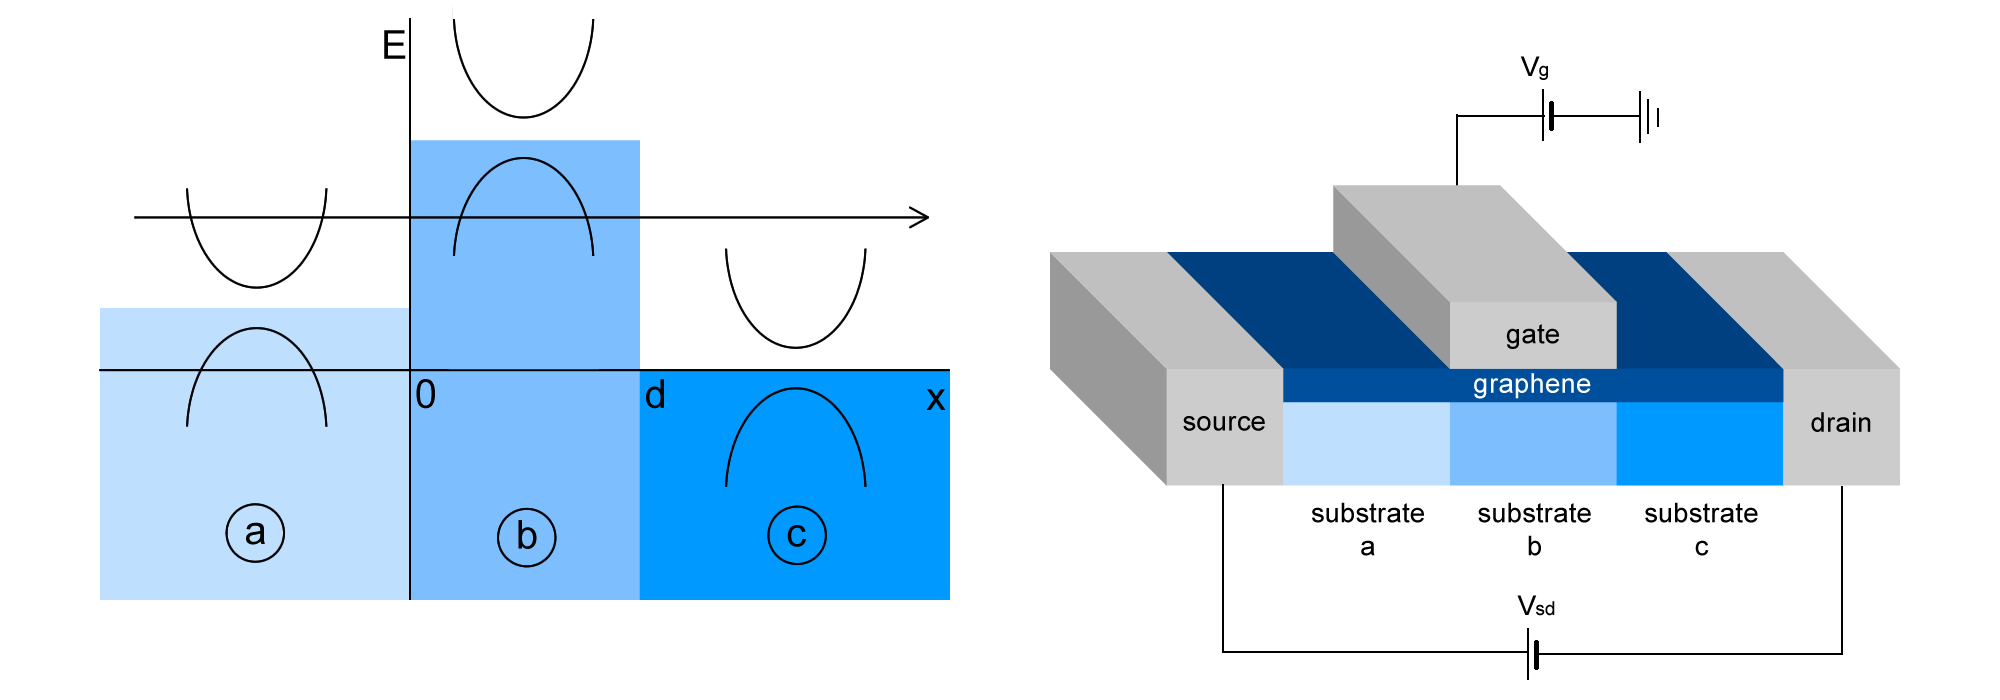
\includegraphics[scale=0.25]{image-abstract-flat}}
		\caption{(Left) Diagram of a Zener tunnelling barrier in graphene, including energy spectrum in specific regions. Here a right travelling massive charge carrier is shown transmitting through a barrier with width $d$ and heights $V_{b}>V_{a}$ and $V_{c}<V_{a}$. (Right) A simple example of a graphene transistor. A third substrate to the right of the gate region creates Zener tunnelling properties.}
		\label{}
	\end{figure}
\end{document}